\section{Literatür Taraması, Özetler ve Pazar Araştırması}
Bu bölüm altında, projenin yapımında kullanılacak teknolojiler, benzer konseptler ve teknik detayların belirlenmesi konusunda yardımcı olacağı düşünülen makalelerin özetlerinden bahsedilmiştir. Ayrıca projenin gerçeklenebilmesi için gereken para ve sürdürülme maliyeti planlanmıştır.
\subsection{E-Posta, SMS ve Push Notification: Hangisi Daha Etkili}
Makalede bahsedilen bildirim kanallarının efektiflikleri karşılaştırılıyor. Bu kanalların hızların, maliyetleri, kullanıcının bildirimi açma oranları gibi faktörler ele alnıyor. Makelde verilen istatiklerin bir kısmı aşşağıdaki tablodan incelenebilir.\cite{socilamediatoday}
\begin{center}
\begin{tabular}{ c | c | c | c }
 Yöntem & E-Posta & SMS & Push Bildirim \\ 
 Ulaşım Süresi & Yavaş & Anında & Anında  \\  
 Açma Oranı & 0.23(Endüstriye Bağlı) & 0.90 & 0.90  \\
 Maliyet & Orta & Yüksek & Düşük \\
 Ulaşılabilirlik & Orta & Yüksek & Orta \\
 Malware Olasığı & Yüksek & Düşük & Düşük \\
 Spam Oranı & Yüksek & Yükse & Düşük \\
 Abonelikten Çıkış Oranı & 0.20-0.50(Endüstriye Bağlı) & 0.60 & 0.40 
\end{tabular}
\end{center}

\subsection{İşletmeler İçin Toplu SMS'in Önemi}
Toplu SMS yöntemleri ile dünyanın her yerine ulaşma imkanı olduğununa değiniliyor. İnsanların \%90'nın gelen SMS'leri ilk 3 saniye içerisinde okuma ihitmalinin aşırı derecede yüksek olduğu söyleniyor. Toplu SMS sistemlerindeki "Aplication-to-Person" (A2P) kullanım kolaylığına dikkat çekiliyor. Özellikle bulut sistemlerindeki entegrasyon kolaylığına değiniliyor.\cite{clickatell} Avantajları 3 madde de özetleyecek olursak:
\begin{itemize}
  \item Global olarak erişim kolaylığı
  \item SMS Fiyatlandırmısanın Avantajları
  \item Kolay sistem entegrasyonu
\end{itemize}
\subsection{API Nedir}
Basit terimler ile Application Programming Interface (API) uygulamaların birbirleriyle etkileşmesini sağlaya yarar. API'ler web tabablı verilere(JSON veya XML) ulaşımda, bu verilerin değiştirilmesinde ve yeni verilen eklenmesinde kullanılır. Misal olarak Twitter'ın API'si sayesinde başka uygulamalardan Twitterin verisine erişim sağlanabilir.\cite{whatisapi}
\subsection{JavaScript Ne İçin Kullanılır}
Java script genelde web tabanlı uygulamar ve web tarayıcılarının programlanmasında kullanılır. Bunların yanısıra sunucularda ve gömülü sistemlerin kontrolünde de kullanılır. Ama en popüler kullanım sebebi web sitesi araclığıyla interaktif bir arayüz sağlanabilmesidir. Ayrıca JavaScript web tarayıcılarının "native" olarak anladığı tek programlama dilidir.\cite{whyjs}
\subsection{Javascript Framework: React}
React açık kaynak bir JavaScript kütüphanesidir ve Single-Page uygulamalar için kullanıcı arayüzü geliştirmede kullanılır. Facebook tarafından ilk defa kullanılmıştır. JSX adı verilen özel bir syntax'ı vardır. Bu syntax sayesinde hem JavaScript vs HTML'i karaşık olarak kullanma imkanı sunar. Hem iOS hem Android hemde Web uygulamarında kodun tekrar kullanımına olanak sağlar.\cite{react}
\subsection{TCP (Transmission Control Protocol) }
TCP bir network üzerindeki cihazlar için bir veri alışverişi standartıdır. 1973'de bilgisayar bilimcisi Robert E. Kahn ve Vinton G. Cerf tarafından bir araştırma makalesinde ilk defa bahsedilmiştir. Son versiyonu 2014 yılında RFC 7324'de\cite{RFC} tanımlanmıştır. TCP'nin şuan kullanımda olan haliyle iki taraflı veri alışverişine olanak sağlar. Tüm veri kayıpları otomatik olarak tespit edilir ve düzeltilir. Bu sebepten dolayı TCP güvenilir protokol olarak adlandırılır. TCP/IP protokol kavramlarıda bütünleşik olarak IP(Internet Protocol)'ünü kasıt ederek kullanılır. 
\newline
\newline
TCP yazılımı web browserler ve sunucular tarfında kontrol edilir. Her bağlantı kaynağı açıkca bitiş noktalarını(end points, server-client) açıkca tanımlamaldır. Hangi tarafın hangi rolü(server yada client) üstenldiği önemli değildir. TCP yazılımına he endpoint için bir çift IP adresi ve port sağlanması yeterlidir(socket ve 2-tuple).\cite{RFC}
\begin{figure}[h]
    \centering
    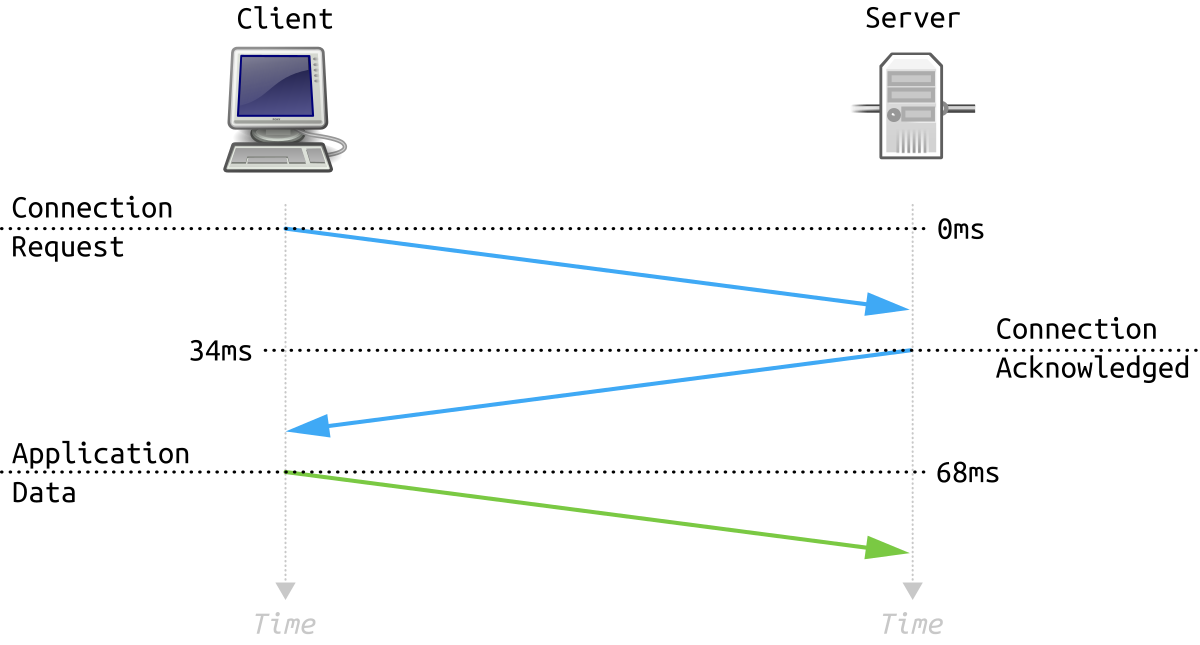
\includegraphics[width=\textwidth]{Report/images/tcp.png}
    \caption{TCP 3-Way Handshake yöntemiyle bağlantı sağlama süreci}
    \label{fig:mesh1}
\end{figure}
\subsection{Websocket Nedir}
Websocket tek bir TCP bağlantısı ile 2 yönlü iletişimi sağlar. Websocket geliştirmek için birçok dil ve kütüphane mevcuttur.\cite{websocket1}
\begin{itemize}
  \item ASP.Net Core: SignalR
  \item Node.js: Socket.IO, ws
  \item WebSockets, ws4py
\end{itemize}
Websocket'ler TCP'nin üzerine kurulan protokollerdir ve ayrıca gerçeklenmesi gerekir. Python'da bu mimariyi gerçekleyen kütüphaneler mevucttur. Yukardıki maddelerde verilen örneklere ek olarak Python'da Tornado kütüphanesi verilebilir\cite{websocket2}.
\subsection{Örnek Bildirim Motoru Mimarisi}
Bu makalade "OracleAS Wireless notification" sistemi mimarisi anlatılıyor. Bu mimari projede gerçeklenecek back-end kısmıyla bazı yönlerden parelellik göstediği için incelendi.
\noindent
Bu mimaride 3 tip bildirim tetikleme yöntemi mevcut.
\begin{itemize}
  \item Veri tetiklemesi
  \item Zaman tetiklemesi
  \item Lokasyon tetiklemsi
\end{itemize}
Veri tetikleme yöntemi bizim sistemimize en uygun olan yöntem. Bu yöntemde kullanıcının belirlediği kurallara göre yeni veri akışı olduğunda bildirim tetikleniyor. Örnek olarak bir hisse senedin belli bir fiyata ulaştığında bildirim gönderilmesi gibi.
\newline
\newline
\noindent
Zaman tetikleme yönteminde ise kullanıcı belirlene bir saatte ve yine isterse belirlediği kurallara göre bildirim alıyor. Örnek olarka kullanıcının her gün saat 15:00 borsa endeksini alması verilebilir.
\newline
\newline
\noindent
Lokasyon tetiklemesi kullanıcın veya kullanıcın takip ettiği kişinin o anki konumunu bir kural olarak kullanarak bildirim sağlanması. Örneğin kullanıcı belli bir dükkanın önündeyse veya işte veya evde değilse trafik durumuyla ilgili bildirim alması verilebilir.
\clearpage
\begin{figure}
    \centering
    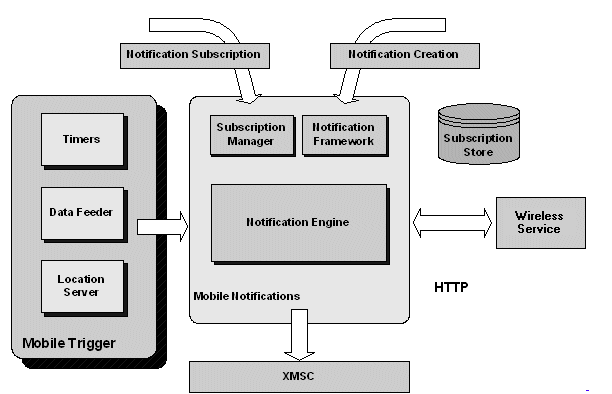
\includegraphics[width=\textwidth]{Report/images/notif.png}
    \caption{Örnek bildirim lojistik mimarisi\cite{notif}}
    \label{fig:mesh2}
\end{figure}
\clearpage
\subsection{Web Uygulamarında Farklı Kimlik Doğrulama Yöntemleri}
Kimlik doğrulama yöntemleri web uygulamalama güvenliğinin sağlanması için gerekli yöntemlerdir. Servise dayalı ve RESTful uygulamarda bu yöntemler şöyle sıralanabilir:
\begin{itemize}
  \item Çerez Tabanlı Kimlik Doğrulama
  \item Token Tabanlı Kimlik Doğrulama
  \item 3. Parti Uygulama Aracılığı ile doğrulama (API, OAuth)
  \item OpenId
  \item SAML (Security assertion markup language)
\end{itemize}
\noindent
Çerez tabanlı doğrulama uzun süreli doğrulama amaçlı kullanılır. Kullanıcı giriş bilgilerini sağladıktan sonra, sunucu(state-full) bir oturum kimliği oluşturur ve bu kimliği kullanıcı ile paylaşır. Kullanıcı çıkış yaptığı takdirde bu kimlik hem sunucudan hem kullanıcan silinir.
\newline
\newline
\noindent
Token tabanlı doğrulama SPA(Single Page Application)'larda yaygın olarak kullanılır. Bu yöntemi gerçeklemenin farklı yolları vardır, en yaygın yolu JSON Web Token(JWT)'dır. Sunucu kullanıcıdan kimlik bilgilerini aldığı zaman bir JWT oluşturur. Bu token sunucu tarafında tutulmaz, sadece kullanıcı tarafında saklanır. Daha sonra gelecek doğrulama istekleri sunucu tarafından onaylanır(decode).
\newline
\newline
\noindent
3. parti uygulama aracılığı uygulama API'sini dışarıya açmak gerektiği durumlarda kullanılır. Örnek olarak Google, Facebook, Twitter kullanıcı doğrulama yöntemleri verilebilir. Bu sağlayıcılar API'lerini genel kullanıma açmıştır. Bu yöntemde güvenlik JWT veya OAuth yardımıyla sağlanır. OAuth'un son sürümü olan OAuth 2.0 Google, Twitter vb. sağlayıcıların HTTPS gerçeklemesine dayanır. Burada bir "Identity Provider" token oluşturur ve güvenliği bunun üzerinden sağlanır.
\newline
\newline
\noindent
OpenID'de yukarıda bahsedilen kimlik sağlayıcı hizmeti veren Google, Facebook, Twitter gibi şirketlerin kimlik sağlayıclarını diğer gelişitiriciler için API yardımıyla kullanımı açılmış halidir. Sitelerde görülen "Facebook ile giriş yap" gibi yöntemler buna örnektir.
\newline
\newline
\noindent
SAML, OpenID(JSON)'nin XML tabanlı versiyonudur. Microsoft servislerinde kullanılır.\cite{auth_medium}
\subsection{Firebase}
Firebase, Google'ın mobil uygulama geliştirme platformudur. İçerisinde istatistik, kimlik doğrulama, veri tabanı, mesajlaşma gibi ihtiyaçları karşılayacak bir alet kutusu gibi nitelendirilebilir. Bulut tabanlıdır. Uygulama ve servis arasında aracı olarak görev yapabilir.
\begin{figure}
    \centering
    \includegraphics[width=\textwidth]{Report/sections/firebase1.png}
    \label{fig:mesh3}
\end{figure}
iOS ve Android Firebase'in uzmanlaştığı platformlardır fakat web, Flutter, Unity ve C++ için de destek vermektedir. Ayrıca diğer dillerde kullanılmak üzere Admin SDK adı verilen paketi mevcuttur.
Firebase Authtentication kullanıcı girişi ve kimlik doğrulamada desteği verir. Nerdeyse tüm kimlik doğrulamaları sistemlerde gerekli olan kullancıya özel verinin saklanması sağlar. Twitter, Google, Faebook, Github sağlayıcılardan(identity provider) tek hesap ile giriş desteği sağlar.
\subsection{Pazar ve Maliyet Araştırması}
Şu an hali hazırda devlet daireleri, belediyeler ve bir çok özel kurum ve kuruluş bilgilendirme yapmak için hem sosyal medya hemde SMS kanallarını kullanmaktadırlar. Günümüzde bilgi güvenliği gündemde sıkça yer bulmaktadır. Facebook, Google, Twitter gibi şirketlerin kullanıcıların onayı dışında özel bilgilere ulaşması konusunda şüpheler mevcuttur. Bu proje kapsamında geliştirilecek sistem sayesinde sosyal medya kanllarından özel bilgilerin tehlikeye atılması söz konusu olmadan yararlanılabilmesini sağlamak ana hedeftir. Toplumsal katkı amaçlı bir sistem olması planlamaktadır.
\newpage
\subsection{Çözüm Yöntemleri}
Sistem gerçeklenmesi kilit taşlardan birisi SMS gönderme yöntemidir. Bu yöntem sistemi maliyeti belirlemektedir. Araştırmalar sonucu makul iki yöntem belirlenmiştir. Bu yöntemlerden ilki donanımsal bir çözümdür. Arduino tipi bir devre ve GSM modülü ile gerçeklenip bu board üzerinde bir bildirim motorunın sürekli olarak çalışması söz konusudur. Bu yöntemin maliyeti 700TL civarı olup, yayınlacak SMS lerin ücereti bu hesaba katılmamıştır.
\newline
\newline
\noindent
İkinci bir yöntem ise yazılımsal bir çözümdür. Bu çözümde 3. parti bir API kullanılarak bir IP numara üzerinde programatik olarak SMS gönderimi sağlanması planlamıştır. Burada donansal bir maliyet yoktur ve SMS maliyeti ilk yöntem ile aynıdır. Sonuç olarak ikinci yöntem hem gerçeklenme açısından kolaylığı hem de maliyet açısında uygulunğu sebebiyle seçilmiştir.




